\documentclass[aspectratio=169,11pt]{beamer}
\usetheme[progressbar=frametitle,numbering=fraction,block=fill]{metropolis}
\usepackage{fontspec}
\setsansfont{Inter}[UprightFont=*-Regular,BoldFont=*-SemiBold,ItalicFont=*-Italic,BoldItalicFont=*-SemiBoldItalic]
\usepackage{pgfplots}
\pgfplotsset{compat=1.18}
\usepackage{tikz}
\usetikzlibrary{positioning}

% Palette: deep ocean + jade + terracotta
\definecolor{ocean}{HTML}{0F2A3D}
\definecolor{jade}{HTML}{1F8A70}
\definecolor{terra}{HTML}{C8553D}
\definecolor{sand}{HTML}{F6F1E9}
\definecolor{ink}{HTML}{1E1E1E}
\definecolor{mute}{HTML}{6B7280}
\setbeamercolor{frametitle}{bg=ocean,fg=white}
\setbeamercolor{normal text}{fg=ink,bg=white}
\setbeamercolor{alerted text}{fg=terra}
\setbeamercolor{progress bar}{fg=jade,bg=ocean!30}
\setbeamercolor{title separator}{fg=jade}
\setbeamercolor{background canvas}{bg=white}
\setbeamercolor{standout}{bg=ocean,fg=white}

\newcommand{\bignum}[2]{\begin{minipage}[t]{\linewidth}\centering{\fontsize{24}{26}\selectfont\bfseries\color{jade}#1}\\[4pt]{\small\color{mute}#2}\end{minipage}}
\newcommand{\src}[1]{\vfill{\scriptsize\color{mute}#1}}

\title{Compute as a Commons}
\subtitle{Mexico, Australia, and the Geography of Discovery}
\author{Jorge Luis Galvez Vallejo}
\institute{National Computational Infrastructure (NCI), Australia}
\date{UNAM \textbullet{} Comparative Social Dynamics: Society, Inequality, and Public Policy}

\begin{document}

% 1 ------------------------------------------------------------
\maketitle

% 2 ------------------------------------------------------------
\begin{frame}{Who gets to ask?}
\begin{center}
{\Large Whoever owns the computing\\[2pt] decides \alert{which questions get asked at all.}}
\end{center}
\vspace{1.2em}
\begin{columns}[T]
\column{0.24\textwidth}\centering{\bfseries\color{ocean}Rivers}\\[2pt]\small Flood forecasting on the Mahanadi, with India's C-DAC
\column{0.24\textwidth}\centering{\bfseries\color{ocean}Coasts}\\[2pt]\small Which shorelines get a storm-surge forecast
\column{0.24\textwidth}\centering{\bfseries\color{ocean}Crops}\\[2pt]\small Which regions get a drought model
\column{0.24\textwidth}\centering{\bfseries\color{ocean}Health}\\[2pt]\small Which diseases get a drug-discovery campaign
\end{columns}
\vspace{1.2em}
\begin{center}\color{mute}Inequality not of income, but of \alert{curiosity}.\end{center}
\end{frame}

% 3 ------------------------------------------------------------
\begin{frame}{Compute is infrastructure}
\begin{center}

\begin{tikzpicture}[node distance=0.5cm,
  box/.style={draw=ocean!40,fill=sand,rounded corners=3pt,minimum width=2.6cm,minimum height=1.1cm,align=center,font=\small},
  hot/.style={box,fill=jade,draw=jade,text=white,font=\small\bfseries}]
\node[box] (a) {Railways\\{\scriptsize\color{mute}19th c.}};
\node[box,right=of a] (b) {Electricity\\{\scriptsize\color{mute}20th c.}};
\node[box,right=of b] (c) {Public universities\\{\scriptsize\color{mute}20th c.}};
\node[hot,right=of c] (d) {Compute + AI\\{\scriptsize 21st c.}};
\draw[->,thick,ocean!50] (a)--(b); \draw[->,thick,ocean!50] (b)--(c); \draw[->,thick,ocean!50] (c)--(d);
\end{tikzpicture}
\end{center}
\vspace{1em}
\begin{columns}[T]
\column{0.3\textwidth}\centering{\Large\bfseries\color{jade}Build}\\\small you set the priorities
\column{0.3\textwidth}\centering{\Large\bfseries\color{ocean}Rent}\\\small someone else sets them
\column{0.3\textwidth}\centering{\Large\bfseries\color{terra}Go without}\\\small your questions wait
\end{columns}
\vspace{1.2em}
\begin{center}\textit{Un bien público.}\end{center}
\end{frame}

% 4 ------------------------------------------------------------
\begin{frame}{Mexico: Coatlicue}
\begin{center}\textit{``La supercomputadora del pueblo''}\end{center}
\vspace{0.6em}
\begin{columns}[T]
\column{0.24\textwidth}\bignum{314 PF}{peak performance}
\column{0.24\textwidth}\bignum{$\sim$14,500}{GPUs}
\column{0.24\textwidth}\bignum{6\,bn}{pesos of public investment}
\column{0.24\textwidth}\bignum{$\sim$7$\times$}{largest system in Latin America}
\end{columns}
\vspace{1.2em}
\small
\begin{itemize}
\item Hub of a national cluster: UNAM, IPN, Cinvestav, BUAP, UAM, and more
\item Staff training at Barcelona Supercomputing Center; technical support from India's C-DAC
\end{itemize}
\src{Source: Secihti / ATDT announcement, Nov 2025, via Xataka México.}
\end{frame}

% 5 ------------------------------------------------------------
\begin{frame}{Australia: ``very far behind''}
\vspace{0.8em}
\begin{columns}[T]
\column{0.32\textwidth}\bignum{2028}{Setonix supported until; no confirmed replacement}
\column{0.32\textwidth}\bignum{4--5$\times$}{cost of a replacement vs.\ the original build}
\column{0.32\textwidth}\bignum{$\sim$3$\times$}{research demand vs.\ available capacity}
\end{columns}
\vspace{1.2em}
\begin{center}
{\large ``A winding down and a closure.''}\\[2pt]{\small\color{mute}Pawsey Supercomputing Research Centre}\\[10pt]
{\large ``Very far behind'' \normalsize on GPUs for AI.}\\[2pt]{\small\color{mute}NCI}
\end{center}
\src{Source: ACS Information Age, 2026.}
\end{frame}

% 6 ------------------------------------------------------------
\begin{frame}{Access follows political decision, not national wealth}
\begin{center}
\begin{tikzpicture}
\begin{axis}[
  xbar, width=0.88\textwidth, height=0.58\textheight,
  xmin=0, xmax=17500,
  ytick={1,2,3,4}, yticklabels={NCI (Australia),Singapore,South Korea,Coatlicue (Mexico)},
  ymin=0.4, ymax=4.6, y dir=reverse,
  bar width=14pt,
  axis x line=none, axis y line*=left, y axis line style={draw=none},
  yticklabel style={font=\small},
  nodes near coords, nodes near coords align={horizontal},
  every node near coord/.append style={font=\small\bfseries},
  /pgf/number format/.cd,1000 sep={{,}},/pgfplots/.cd,
  major tick length=0pt,
]
\addplot[fill=ocean!35,draw=none,bar shift=0pt] coordinates {(120,1) (1500,2) (8500,3)};
\addplot[fill=jade,draw=none,bar shift=0pt] coordinates {(14500,4)};
\end{axis}
\end{tikzpicture}
\end{center}
\vspace{-0.6em}
\begin{center}\small GPUs for public research. Mexico is about to have \alert{more than 100$\times$} Australia's national facility.\end{center}
\src{NCI: latest-generation GPUs. Coatlicue: planned. Sources: ACS Information Age 2026; Xataka México 2025.}
\end{frame}

% 7 ------------------------------------------------------------
\begin{frame}{A machine is not enough}
\begin{columns}[T]
\column{0.31\textwidth}
{\Large\bfseries\color{jade}People}\\[4pt]
\small Specialists to run it, scientists to use it, and a reason to stay when industry pays more.
\column{0.31\textwidth}
{\Large\bfseries\color{jade}Governance}\\[4pt]
\small Science, Pemex, tax, industry: who sets the shares? Oaxaca vs.\ Mexico City; regions vs.\ the capital.
\column{0.31\textwidth}
{\Large\bfseries\color{jade}Continuity}\\[4pt]
\small Machines age in 5--6 years. A permanent public service, not a one-off purchase.
\end{columns}
\vspace{1.5em}
\begin{center}\color{mute}A public machine with closed allocation rules just moves the queue indoors.\end{center}
\end{frame}

% 8 ------------------------------------------------------------
\begin{frame}{Compute as a commons: a Mexico--Australia proposal}
\begin{columns}[T]
\column{0.36\textwidth}
{\bfseries\color{ocean}Three layers}
\begin{itemize}\small
\item \textbf{Machines}, publicly owned
\item \textbf{Code}, openly shared
\item \textbf{People}, trained and kept
\end{itemize}
\vspace{0.3em}
{\small\color{mute}One ocean: cyclones, floods, reefs, drought, rising seas.}
\column{0.58\textwidth}
{\bfseries\color{ocean}Three proposals}
\begin{enumerate}\small
\item \textbf{Pacific modelling partnership:} joint ocean, climate and flood forecasting on both nations' public machines
\item \textbf{People exchange:} engineers and students between Coatlicue and Australia's national facilities
\item \textbf{Shared open code:} built once, adapted to the Usumacinta or the Murray--Darling
\end{enumerate}
\end{columns}
\vspace{0.3em}
\begin{center}
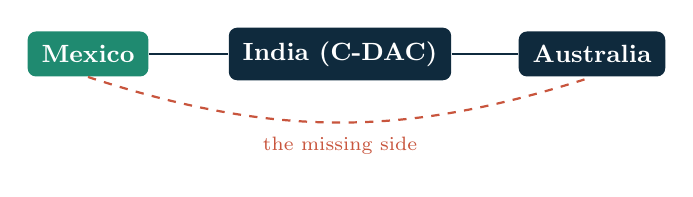
\begin{tikzpicture}[every node/.style={font=\small\bfseries,text=white,rounded corners=3pt,inner sep=5pt}]
\node[fill=jade] (mx) at (0,0) {Mexico};
\node[fill=ocean] (in) at (3.2,0) {India (C-DAC)};
\node[fill=ocean] (au) at (6.4,0) {Australia};
\draw[thick,ocean] (mx)--(in); \draw[thick,ocean] (in)--(au);
\draw[thick,terra,dashed] (mx.south) to[bend right=18] node[below,text=terra,font=\scriptsize]{the missing side} (au.south);
\end{tikzpicture}
\end{center}
\end{frame}

% 9 ------------------------------------------------------------
\begin{frame}[standout]
Not closing doors.\\[6pt]
Owning a door of your own,\\ and leaving it open.\\[18pt]
{\normalsize Gracias}
\end{frame}

\end{document}
